% Working note, version 2 (English).  Build from docs/:  latexmk -lualatex SignoriniPostprocessing_v2.tex
% Figures are read from ../results/pdf/.
\documentclass[11pt,a4paper]{article}

\usepackage{fontspec}
\usepackage[english]{babel}
\usepackage{amsmath,amssymb,amsthm}
\usepackage[margin=2.4cm]{geometry}
\usepackage{booktabs}
\usepackage{graphicx}
\usepackage[font=small,labelfont=bf]{caption}
\usepackage[section]{placeins}
\usepackage[hidelinks]{hyperref}

\graphicspath{{../results/pdf/}}
\setlength{\emergencystretch}{3em}

\theoremstyle{definition}
\newtheorem{definition}{Definition}[section]
\newtheorem{remark}[definition]{Remark}
\newtheorem{proposition}[definition]{Proposition}

\newcommand{\BDM}{\mathrm{BDM}}
\newcommand{\Pk}[1]{\mathrm{P}_{#1}}
\newcommand{\dive}{\operatorname{div}}
\newcommand{\jmp}[1]{[\![#1]\!]}
\newcommand{\Th}{\mathcal{T}_h}
\newcommand{\Fi}{\mathcal{F}^{i}_h}
\newcommand{\FD}{\mathcal{F}^{D}_h}
\newcommand{\FC}{\mathcal{F}^{C}_h}

\title{Scalar Signorini in dual-mixed form on a Bernstein cone:\\
MRV postprocessing and a contact-boundary estimator}
\author{Working note}
\date{November 13, 2026 (version 2)}

\begin{document}
\maketitle

\begin{abstract}
The scalar Signorini problem is discretised in dual-mixed form with $\BDM_{k+1}\times\Pk{k}$,
\mbox{$k=0,\dots,3$}, without a Lagrange multiplier: the sign of the normal flux is imposed on the
Bernstein coefficients of its trace on each contact edge, and the resulting variational inequality
is solved by a primal-dual active set acting coefficient by coefficient. The solution is
postprocessed with the local residual minimisation of Muga--Rojas--Vega (MRV)~\cite{mrv}, and an a
posteriori indicator is built from the improved MRV estimator plus a contact-boundary term weighted
by the Bernstein partition of unity of the discrete active set. The indicator does not use the
equilibrium equation. Its reliability is not proved; everything said about it here is numerical.
The experiments cover manufactured solutions with smooth and singular transition points, the
problem without contact as a control, and the examples of Führer--Heuer--Stephan~\cite{fhs} and
Bartels--Gudi--Kaltenbach~\cite{bgk}.
\end{abstract}

\paragraph{Changes with respect to version 1.}
\begin{itemize}
  \item The two open questions on the indicator (Section~\ref{sec:open}) are stated as hypotheses
        with the evidence for and against them. Version 1 stated as facts that (i) an indicator that
        does not use the equilibrium equation cannot see the oscillation of $f$, and (ii) with the
        transition point inside an edge the missing error is contact error that no term captures and
        that adaptivity removes. A new control experiment, the same solution without contact (E5),
        shows that part of (ii) is not a contact effect.
  \item Corrected details: the edge-wise classification also improves on having no contact term;
        the complementarity term overestimates by up to $\sim\!50$ (not $\sim\!30$); the contact
        term follows the contact-zone trace error within a factor $0.97$--$2.2$; Theorem~3.9
        of~\cite{mrv} needs the saturation assumption also for the linear problem.
  \item Every claim on the indicator is backed by a table or a figure.
\end{itemize}

\section{Problem and notation}

Let $\Omega\subset\mathbb{R}^2$ be a polygon with $\partial\Omega=\Gamma_D\cup\Gamma_C$,
$\Gamma_D\cap\Gamma_C=\emptyset$, $|\Gamma_D|>0$, and let $f\in L^2(\Omega)$, $u_D\in
H^{1/2}(\Gamma_D)$. The problem is
\begin{equation}\label{eq:problem}
  -\Delta u=f \ \text{in }\Omega,\qquad u=u_D \ \text{on }\Gamma_D,\qquad
  u\ge0,\quad \partial_nu\ge0,\quad u\,\partial_nu=0 \ \text{on }\Gamma_C .
\end{equation}
We write $\sigma:=\nabla u$, so that $\dive\sigma=-f$ and the sign condition reads
$\sigma\cdot n\ge0$ on $\Gamma_C$ (dual-mixed form as in~\cite{wang}); in the notation
of~\cite{mrv}, $q:=-\sigma$. The contact set is
$\Gamma_C^0:=\{u=0\}\subset\Gamma_C$ and a \emph{transition point} is an endpoint of
$\Gamma_C^0$ in the relative interior of $\Gamma_C$.

$\Th$ is a shape-regular triangulation compatible with $\Gamma_D/\Gamma_C$; $\Fi,\FD,\FC$ are the
interior edges and the edges on $\Gamma_D$ and $\Gamma_C$, and $K_E$ is the element containing
$E\in\FC$. For $E\in\FC$ and $g\in\Pk{m}(E)$, $b_{E,i}(g)$, $i=0,\dots,m$, are the degree-$m$
Bernstein coefficients of $g$ and $B_{E,i}$ the Bernstein basis, so that
$g=\sum_ib_{E,i}(g)\,B_{E,i}$, $B_{E,i}\ge0$, $\sum_iB_{E,i}=1$.

\begin{remark}[obstacle, Neumann, reaction]\label{rem:variants}
With an obstacle $u\ge\chi$ on $\Gamma_C$, a homogeneous Neumann part $\Gamma_N$
($\sigma\cdot n=0$) and a reaction term $-\Delta u+cu=f$, $c\ge0$, everything below holds after
replacing $u$ and $\nu_h$ by $u-\chi$ and $\nu_h-\chi$ on $\Gamma_C$, imposing $\sigma_h\cdot n=0$
on $\Gamma_N$, and adding $-(c\,u_h,v)$ to the equilibrium equation. If $c>0$, $\Gamma_D$ may be
empty (the examples of~\cite{fhs} have $c=1$ and Signorini conditions on all of $\partial\Omega$).
\end{remark}

\section{Mixed solution}

Let $\Sigma_h=\BDM_{k+1}$ and $Q_h=\Pk{k}(\Th)$, $k\ge0$ (MRV's $p$ is $k+1$). The normal trace of
$\tau\in\Sigma_h$ on $E\in\FC$ lies in $\Pk{k+1}(E)$ and is fixed by the $k+2$ degrees of freedom
of $E$. The discrete cone is
\[
  K_h:=\{\tau\in\Sigma_h:\ b_{E,i}(\tau\cdot n|_E)\ge0\quad\forall E\in\FC,\ i=0,\dots,k+1\},
\]
and $(\sigma_h,u_h)\in K_h\times Q_h$ solves
\begin{equation}\label{eq:mvi}
  (\sigma_h,\tau-\sigma_h)+(u_h,\dive(\tau-\sigma_h))\ge\langle u_D,(\tau-\sigma_h)\cdot n\rangle_{\Gamma_D}
  \quad\forall\tau\in K_h,\qquad (\dive\sigma_h,v)=-(f,v)\quad\forall v\in Q_h .
\end{equation}
Since the Bernstein basis is non-negative, $\tau\in K_h$ implies $\tau\cdot n\ge0$ pointwise on
$\Gamma_C$. For $k=0$ the condition is also necessary (the trace is linear and its coefficients are
its end values); for $k\ge1$ it is only sufficient. Hence $\sigma_h$ satisfies the sign condition at
every point, and $\dive\sigma_h=-Q_hf$ with $Q_h$ the $L^2$ projection onto $\Pk{k}(\Th)$.

\begin{remark}[cone without multiplier]
On each $E\in\FC$ the $k+2$ degrees of freedom of $\sigma_h\cdot n|_E$ are replaced by its
Bernstein coefficients $c_{E,i}$ through a fixed $(k+2)\times(k+2)$ matrix, computed from the
values of the basis at the Bernstein nodes. Each coefficient is either \emph{in contact} (free)
or \emph{separated} ($c_{E,i}=0$). This is a linear change of variables $x=T\tilde x$ applied to the
assembled saddle-point system, and no Lagrange multiplier is introduced.
\end{remark}

\begin{remark}[active set]\label{rem:pdas}
The multiplier of $c_{E,i}\ge0$ is $\mu_{E,i}:=\bigl[T^\top(Kx-b)\bigr]_{E,i}$, the residual of the
full system in the direction of the flux whose normal trace on $E$ is $B_{E,i}$; its continuous
counterpart is $\int_E u\,B_{E,i}$. The KKT conditions of~\eqref{eq:mvi} are $c\ge0$, $\mu\ge0$,
$c_{E,i}\mu_{E,i}=0$, and the primal-dual active set update is
\[
  \text{contact}\to\text{separated if } c_{E,i}<-\mathrm{tol}\,\|c\|_\infty,\qquad
  \text{separated}\to\text{contact if } \mu_{E,i}<-\mathrm{tol}\,\|\mu\|_\infty,
\]
with $\mathrm{tol}=10^{-10}$ (cf.~\cite{hik}). It terminated in all runs, in at most $44$ iterations ($k=3$,
$N\approx5\cdot10^4$), starting from the fully separated state. We write
$\beta_E:=\sum_{i\ \text{in contact}}B_{E,i}$, the Bernstein partition of unity restricted to the
coefficients in contact; $\beta_E\equiv1$ on an edge fully in contact, $\beta_E\equiv0$ on a
separated one, and in between on an edge that a transition point cuts.
\end{remark}

\section{Postprocessing}

With $q_h:=-\sigma_h$, on each $K\in\Th$ the MRV problem~\cite[(3.2)]{mrv} reads: find
$(\varepsilon_K,\nu_K)\in V^{k+3}_{\star,K}\times V^{k+2}_K$ with
\begin{equation}\label{eq:mrv}
\begin{aligned}
  (\nabla\varepsilon_K+\nabla\nu_K,\nabla v)_K&=-(q_h,\nabla v)_K &&\forall v\in V^{k+3}_{\star,K},\\
  (\nabla w,\nabla\varepsilon_K)_K&=0 &&\forall w\in V^{k+2}_{\star,K},\qquad (\nu_K,1)_K=(u_h,1)_K,
\end{aligned}
\end{equation}
where $V^r_K=\Pk{r}(K)$ and $V^r_{\star,K}$ its zero-mean subspace. We write $\nu_h|_K:=\nu_K$,
$\varepsilon_h|_K:=\varepsilon_K$ and $\tilde\eta_K:=\|\nabla\varepsilon_K\|_K$. The
postprocessing is not constrained on $\Gamma_C$: $\nu_h\ge0$ may fail there.

\begin{remark}[Stenberg]
By~\cite[Prop.~3.1]{mrv}, $\nu_h$ coincides with the (modified) Stenberg postprocessing
\cite[(2.10)]{mrv}. Both were computed independently on the meshes of E1: the relative difference is
at most $5\cdot10^{-15}$ in $L^2$ and $10^{-13}$ in the broken $H^1$ seminorm, for $k=0,\dots,3$.
\end{remark}

\section{Indicator}

\begin{definition}\label{def:eta}
For $K\in\Th$,
\begin{align*}
  \eta_K^2:={}& \tilde\eta_K^2+\|\sigma_h-\nabla\nu_K\|_K^2
   +\tfrac12\sum_{F\in\mathcal{F}^i_K}h_F^{-1}\|\jmp{\nu_h}\|_F^2
   +\sum_{F\in\mathcal{F}^D_K}h_F^{-1}\|u_D-\nu_h\|_F^2 \\
  &+\sum_{E\in\mathcal{F}^C_K}\Bigl(h_E^{-1}\|\beta_E^{1/2}\,\nu_h\|_E^2
     +h_E^{-1}\|(1-\beta_E)^{1/2}\min(\nu_h,0)\|_E^2\Bigr),
\end{align*}
and $\eta^2:=\sum_K\eta_K^2$. With an obstacle, $\nu_h$ is replaced by $\nu_h-\chi$ in the last two
terms (Remark~\ref{rem:variants}).
\end{definition}

On $\Gamma_C$ the trace of $u$ is unknown, and the Dirichlet term of~\cite[(3.9)]{mrv} is replaced by
a trace term where the discrete active set says contact ($u=0$) and by the violation of $u\ge0$
where it says separation. Table~\ref{tab:mrv} compares the terms with those of MRV.

\begin{table}[h]
\centering\small
\begin{tabular}{@{}lll@{}}
\toprule
term & MRV, estimator (3.9) & this note \\
\midrule
$\tilde\eta_K=\|\nabla\varepsilon_K\|_K$ & yes & yes \\
$\|q_h+\nabla\nu_K\|_K=\|\sigma_h-\nabla\nu_K\|_K$ & yes & yes \\
jumps $h_F^{-1}\|\jmp{\nu_h}\|_F^2$ & yes & yes \\
Dirichlet $h_F^{-1}\|u_D-\nu_h\|_F^2$ & yes & yes \\
contact boundary & absent & $\beta_E$-weighted trace and $\min(\nu_h,0)$ \\
sign of $\sigma_h\cdot n$ & absent & not needed: $\sigma_h\cdot n\ge0$ pointwise \\
equilibrium residual / oscillation & $\mathrm{osc}(q)$, via Fortin & not used \\
\bottomrule
\end{tabular}
\caption{Comparison with the improved estimator (3.9) of~\cite{mrv}.}
\label{tab:mrv}
\end{table}

\begin{remark}[what is not included]\label{rem:notincluded}
(a) No equilibrium residual: the indicator uses only the constitutive law $q=-\nabla u$, the
conformity of $\nu_h$ and the boundary conditions, as MRV's. (b) No complementarity term
$|\langle\sigma_h\cdot n,\nu_h\rangle_E|$: it is the product of an $O(1)$ factor and an
$O(\text{error})$ factor, not quadratic in the error, and it overestimates more and more as $k$
grows (Section~\ref{sec:choice}). (c) No term on $\Gamma_N$, where $\sigma_h\cdot n=0$ is exact.
\end{remark}

\begin{remark}[reliability]
Reliability for the variational inequality is not proved. Even for the linear problem,
Theorem~3.9 of~\cite{mrv} gives it under the saturation assumption (Assumption~3.5), with constant
$1/(1-\delta)$, where $\delta:=\|\nabla_h(u-\theta_h)\|/\|\nabla_h(u-\nu_h)\|$ and $\theta_h$ is the
Stenberg postprocessing of degree $k+3$~\cite[(3.3)]{mrv}.
\end{remark}

\section{Error measures}

The error of the postprocessing is measured in the MRV norm with jumps, with a trace term only
where the trace of $u$ is prescribed:
\[
  E_s^2:=\|\sigma-\sigma_h\|^2+\|\nabla_h(u-\nu_h)\|^2+\sum_{F\in\Fi}h_F^{-1}\|\jmp{\nu_h}\|_F^2
  +\sum_{F\in\FD}h_F^{-1}\|u-\nu_h\|_F^2+\sum_{E\in\FC}h_E^{-1}\|u-\nu_h\|_{E\cap\Gamma_C^0}^2 .
\]
On the separated part of $\Gamma_C$, as on $\Gamma_N$, the trace of $u$ is not prescribed and the norm
carries no trace term. The built-in indicator $\tilde\eta=(\sum_K\tilde\eta_K^2)^{1/2}$ is measured
against its own norm~\cite[Thm.~3.6]{mrv}, $E^2:=\|\nabla_h(u-\nu_h)\|^2+\|q-q_h\|_*^2$, where
$\|\cdot\|_*$ is the discrete dual norm over $\nabla V^{k+3}_{\star,K}$, computed exactly through its
local Riesz representative. Effectivities are $\eta/E_s$ and $\tilde\eta/E$.

\section{Numerical experiments}\label{sec:num}

\paragraph{Implementation.} Julia prototype on Gridap, with $\BDM_{k+1}\times\Pk{k}$, $k=0,\dots,3$,
on meshes of right triangles (each square of a Cartesian grid split along one diagonal). Uniform
refinement halves $h$; adaptive refinement uses Dörfler marking ($\theta=1/2$) on $\eta_K^2$ and
newest-vertex bisection. The local problems~\eqref{eq:mrv} are solved densely element by element.
$N$ is the number of degrees of freedom of the mixed problem. Rates are least-squares slopes over the
last decade of $N$, reported as $e\sim N^{s}$ (in 2D, $h\sim N^{-1/2}$); effectivity ranges are over
the same decade.

\paragraph{Examples.} $u_s:=-r^{\alpha}\sin(\alpha\theta)$ in polar coordinates centred at
$(x_0,0)$, $\theta\in[0,\pi]$; on $y=0$ it has contact for $x>x_0$ and separation for $x<x_0$.
\begin{itemize}
  \item[E1] $u=u_s+y^2$, $\alpha=11/2$, $x_0=0$, on $(-\frac12,\frac12)\times(0,1)$, $\Gamma_C$ the bottom,
        exact Dirichlet data elsewhere, $f=-2$. Smooth: $u\in H^{13/2-\epsilon}$.
  \item[E2] As E1 with $\alpha=3/2$: $u\in H^{5/2-\epsilon}$, the generic Signorini regularity at a
        transition point. $x_0=0$ is a node of every mesh.
  \item[E3] As E2 with $x_0=1/(2\pi)$: irrational, so never a node of these dyadic meshes; the
        transition always lies inside an edge.
  \item[E4] E3 plus $L=0.3x-0.05$, with obstacle $\chi=L$ on $\Gamma_C$ ($L$ is harmonic and
        $\partial_yL=0$, so $u-\chi$ and $\sigma\cdot n$ on $\Gamma_C$ are those of E3).
  \item[E5] Control: the solutions of E2 and E3 \emph{without contact} (Dirichlet data on the whole
        boundary), with the same indicator (it reduces to MRV's (3.9)).
  \item[E6] FHS 4.2~\cite{fhs}: $-\Delta u+u=f$ on $(-1,1)\times(0,1)$, Signorini on all of
        $\partial\Omega$, piecewise polynomial $u$; mesh aligned with $x=0$, transitions at nodes.
  \item[E7] FHS 4.3~\cite{fhs}: L-shaped domain, $-\Delta u+u=f$, $f=-1$ for $|x|\le0.8$ and $\frac12$
        else, Signorini on all of $\partial\Omega$. No exact solution.
  \item[E8] BGK 7.2~\cite{bgk}: $(0,1)^2$, $u=-10\,\psi(r)\,r^{3/2}\sin(\frac32\theta)$ centred at
        $(\frac12,0)$, $\psi$ the $C^4$ cut-off of degree 9 on $[0,0.45]$; $f\notin\Pk{k}$ with large
        gradients. The transition is a node.
  \item[E9] BGK 7.3.1~\cite{bgk}: $(-1,1)^2$, $f=-1$, obstacle $\chi=\min\{\frac12(|x_1|-\frac12),0\}$
        at the bottom, Dirichlet at the top and on $\{1\}\times(0,1)$, Neumann elsewhere. No exact
        solution.
\end{itemize}
FHS 4.4 (singularly perturbed) is not reproduced: its manufactured solution, as printed, does not
satisfy the Signorini conditions on $x=1$ (there $u>0$ and $\partial_nu\ne0$).

\subsection{Convergence and superconvergence}\label{sec:conv}

Table~\ref{tab:e1} (E1). The rates are optimal for $\sigma_h$ and $u_h$, and $\nu_h$ gains two
orders for every $k$, also for $k=0$ because $f\in\Pk0$ (Section~\ref{sec:low}). The transition is
smooth here ($u_s\sim r^{11/2}$).

\begin{table}[htbp]
\centering\small
\begin{tabular}{@{}lcccc@{}}
\toprule
$k$ & $\|\sigma-\sigma_h\|$ & $\|u-u_h\|$ & $\|u-\nu_h\|$ & finest $h$ \\
\midrule
0 & 1.99 & 1.00 & 2.99 & 1/64 \\
1 & 2.99 & 2.00 & 4.00 & 1/32 \\
2 & 4.00 & 3.00 & 5.01 & 1/32 \\
3 & 5.23 & 4.00 & 6.02 & 1/16 \\
\bottomrule
\end{tabular}
\caption{E1, uniform refinement: rates with respect to $h$ on the two finest meshes.}
\label{tab:e1}
\end{table}

\subsection{Singular solutions and adaptivity}\label{sec:adapt}

Table~\ref{tab:adapt}, Figure~\ref{fig:e3k2}. Uniform refinement is limited by
$u\in H^{5/2-\epsilon}$ to $N^{-3/4}$ for $\sigma_h$ and $N^{-5/4}$ for $\nu_h$ (E2); in E3 the
uniform errors oscillate with the relative position of $x_0$ in its edge. Adaptive refinement driven
by $\eta$ recovers the optimal rates, including the superconvergence of $\nu_h$, for every $k$. The
contact terms are $0.03$--$1.1\,\%$ of $\eta^2$ on the last adaptive mesh: the indicator is
dominated by $\|\sigma_h-\nabla\nu_h\|$.

\begin{table}[htbp]
\centering\small
\begin{tabular}{@{}lcccccc@{}}
\toprule
 & \multicolumn{3}{c}{E2 ($x_0=0$)} & \multicolumn{3}{c}{E3 ($x_0=1/(2\pi)$)} \\
\cmidrule(lr){2-4}\cmidrule(lr){5-7}
$k$ & $\|\sigma-\sigma_h\|$ & $\|u-\nu_h\|$ & $\eta$ & $\|\sigma-\sigma_h\|$ & $\|u-\nu_h\|$ & $\eta$ \\
\midrule
0 & $-1.00$ & $-1.49$ & $-1.00$ & $-1.01$ & $-1.51$ & $-1.01$ \\
1 & $-1.51$ & $-2.01$ & $-1.51$ & $-1.51$ & $-2.02$ & $-1.51$ \\
2 & $-2.03$ & $-2.57$ & $-2.03$ & $-2.04$ & $-2.57$ & $-2.03$ \\
3 & $-2.57$ & $-3.07$ & $-2.56$ & $-2.65$ & $-3.17$ & $-2.62$ \\
\midrule
uniform & $-0.75$ & $-1.25$ & $-0.75$ & \multicolumn{3}{c}{oscillating} \\
\bottomrule
\end{tabular}
\caption{E2 and E3, adaptive refinement driven by $\eta$: slopes $s$ in $e\sim N^s$. Optimal:
$-(k+2)/2$ for $\sigma$ and $\eta$, $-(k+3)/2$ for $\nu_h$.}
\label{tab:adapt}
\end{table}

\begin{figure}[htbp]
  \centering
  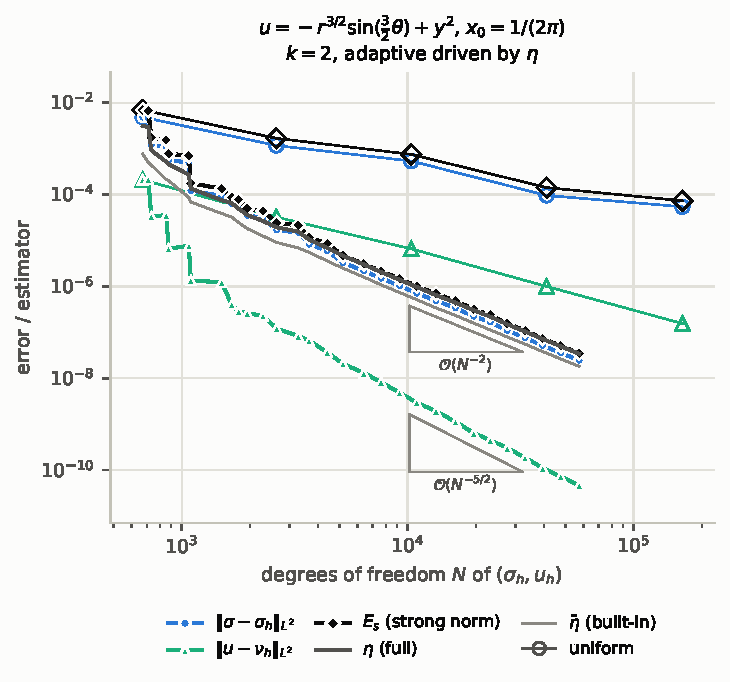
\includegraphics[width=0.58\linewidth]{06_estimators/offset_k2.pdf}
  \caption{E3, $k=2$: errors, $\eta$ and $\tilde\eta$ against $N$; $\eta$-driven adaptive (filled)
  and uniform (hollow) refinement.}
  \label{fig:e3k2}
\end{figure}

\subsection{Choice of the contact term}\label{sec:choice}

On the same solutions of E2--E4 (all with $f\in\Pk0$, so nothing but the contact can be missed),
the contact term of Definition~\ref{def:eta} (B) was replaced by: (A) nothing; (Bf) the same with
an edge-wise classification (an edge is in contact iff all its coefficients are) instead of
$\beta_E$; (Bs) the same with contact where $\sigma_h\cdot n>0$; (C) B plus
$|\langle\sigma_h\cdot n,\nu_h\rangle_E|$; (D) B plus $h_E\|\sigma_h\cdot n\|^2_{E\cap\{\nu_h>0\}}$.

Table~\ref{tab:variants}, Figures~\ref{fig:variants} and~\ref{fig:ratio}. With the transition at a
node all variants except C and D coincide: the active set resolves the contact and the term barely
matters. With the transition inside an edge and uniform refinement, B improves on A (for $k=3$, per
level, from $0.23$--$0.47$ to $0.41$--$0.50$), Bf improves less, Bs is noisy because
$\sigma_h\cdot n$ is close to zero near the transition, C grows with $k$ as expected from its order,
and D is useless. The contact term of B follows the trace error on the exact contact zone within a
factor $0.97$--$2.2$. E4 gives the same numbers as E3, which checks the treatment of $\chi$.

\begin{table}[htbp]
\centering\small
\begin{tabular}{@{}lccc@{}}
\toprule
variant & E2, adaptive & E3, adaptive & E3, uniform \\
\midrule
A  none                                     & 0.67--1.03 & 0.65--1.02 & 0.26--0.80 \\
B  Definition~\ref{def:eta}                 & 0.67--1.03 & 0.67--1.02 & 0.47--0.83 \\
Bf edge-wise classification                 & $\approx$ B & $\approx$ B & 0.34--0.83 \\
Bs classification by $\sigma_h\cdot n>0$    & $\approx$ B & 0.67--4.45 & 0.63--2.58 \\
C  B + complementarity                      & 0.68--34   & 0.68--29 (E4: 51) & 0.49--1.14 \\
D  B + flux where $\nu_h>0$                 & $3\cdot10^2$--$2\cdot10^7$ & $2\cdot10^2$--$10^7$ & $7\cdot10^1$--$5\cdot10^2$ \\
\bottomrule
\end{tabular}
\caption{$\eta/E_s$ for the contact-term variants, $k=0,\dots,3$ together.}
\label{tab:variants}
\end{table}

\begin{figure}[htbp]
  \centering
  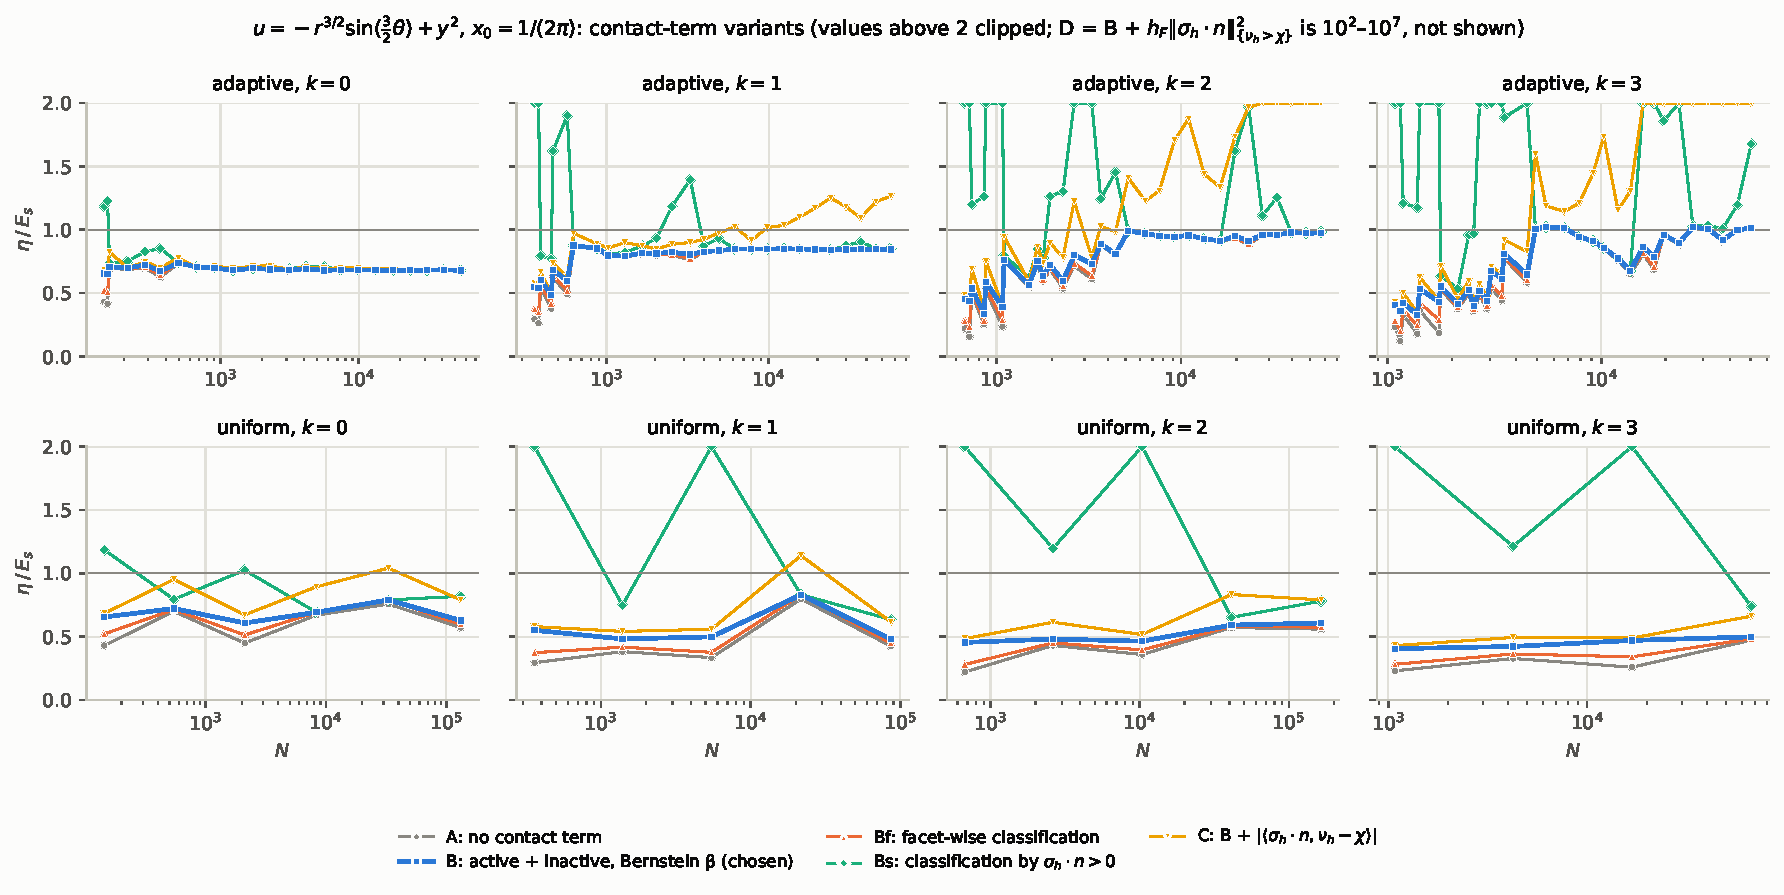
\includegraphics[width=\linewidth]{06_estimators/contact_variants_offset.pdf}
  \caption{E3: $\eta/E_s$ for the variants A, B, Bf, Bs and C; adaptive (top) and uniform (bottom)
  refinement; values above 2 are clipped.}
  \label{fig:variants}
\end{figure}

\begin{figure}[htbp]
  \centering
  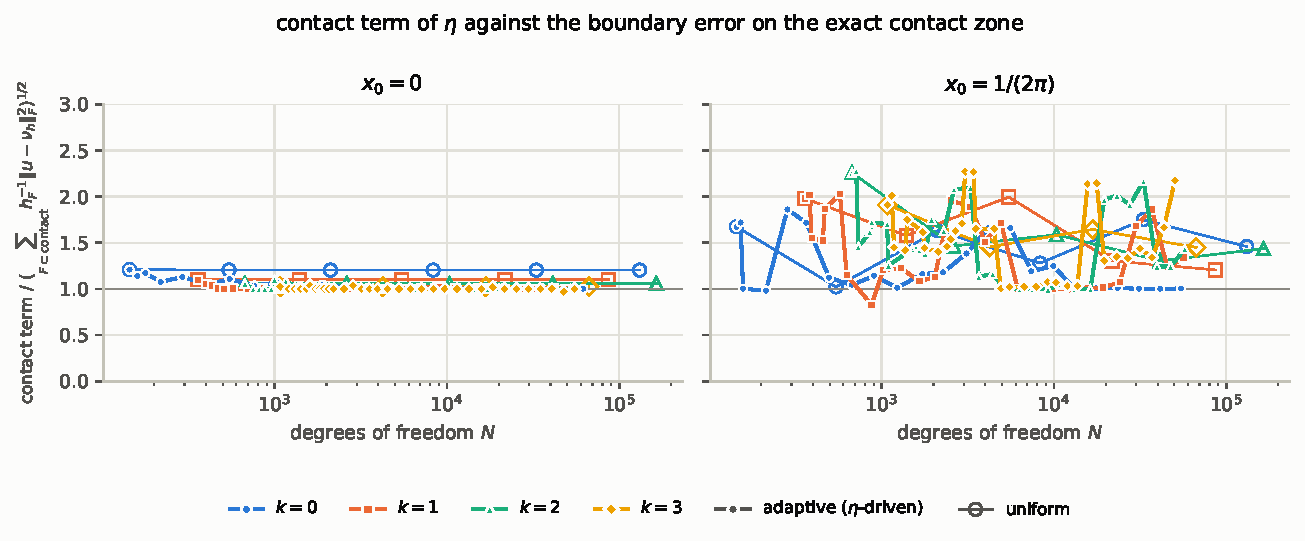
\includegraphics[width=0.92\linewidth]{06_estimators/contact_ratio.pdf}
  \caption{E2 (left) and E3 (right): contact term of $\eta$ divided by the trace error on the exact
  contact zone, $(\sum_E h_E^{-1}\|u-\nu_h\|^2_{E\cap\Gamma_C^0})^{1/2}$.}
  \label{fig:ratio}
\end{figure}

\subsection{Effectivity}\label{sec:eff}

Table~\ref{tab:eff}, Figure~\ref{fig:eff}. Compared with $\tilde\eta$, $\eta$ roughly doubles the
effectivity, approaches $1$ for $k\ge2$ under adaptive refinement, and converges at the rate of
$E_s$.

\begin{table}[htbp]
\centering\small
\begin{tabular}{@{}lccc@{}}
\toprule
example & $\eta/E_s$ adaptive & $\eta/E_s$ uniform & $\tilde\eta/E$ adaptive \\
\midrule
E2 ($x_0$ a node)                    & 0.67--1.03 & 0.64--0.73 & 0.31--0.75 \\
E5, same $u$ without contact          & 0.67--1.03 & 0.64--0.73 & -- \\
E3 ($x_0$ inside an edge)             & 0.67--1.02 & 0.47--0.83 & 0.31--0.73 \\
E5, same $u$ without contact          & 0.68--1.03 & 0.63--0.76 & -- \\
E6, FHS 4.2 ($k\le2$)                 & 0.24--0.74 & 0.63--0.79 & 0.09--0.46 \\
E8, BGK 7.2                          & 0.20--0.32 & 0.35--0.73 & 0.08--0.17 \\
\bottomrule
\end{tabular}
\caption{Effectivities, $k=0,\dots,3$ together.}
\label{tab:eff}
\end{table}

\begin{figure}[htbp]
  \centering
  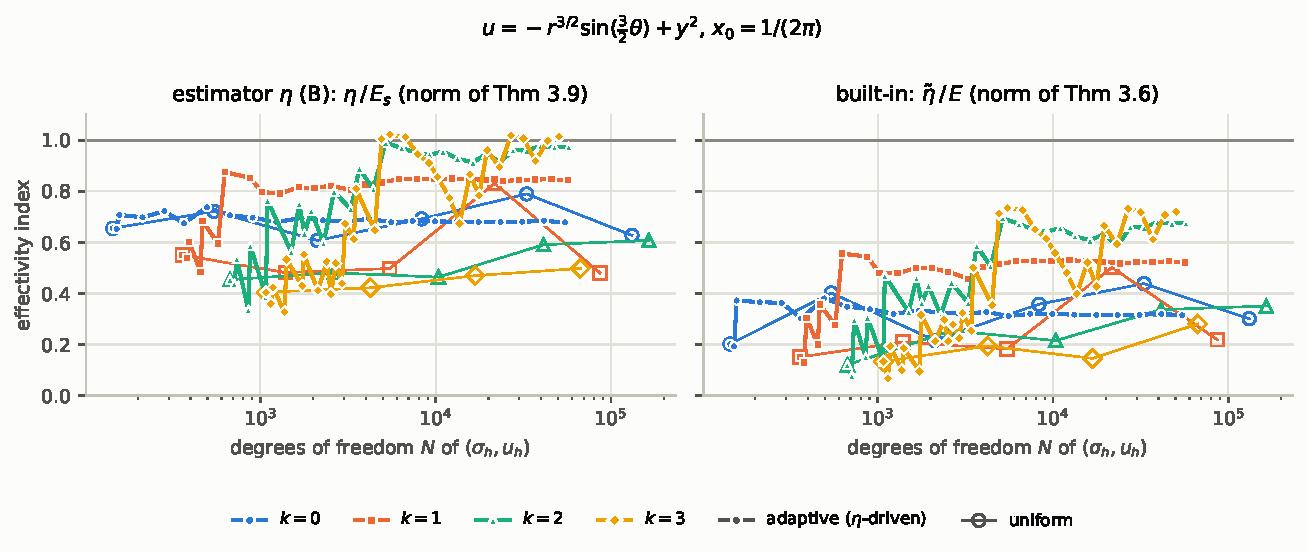
\includegraphics[width=\linewidth]{06_estimators/offset_effectivity.pdf}
  \caption{E3: $\eta/E_s$ (left) and $\tilde\eta/E$ (right); $\eta$-driven adaptive (filled) and
  uniform (hollow) refinement.}
  \label{fig:eff}
\end{figure}

\subsection{Contact or singularity: the control without contact}\label{sec:control}

Table~\ref{tab:linear}, Figure~\ref{fig:linear}. With the transition at a node, Signorini and the
problem without contact give the same effectivities. With the transition inside an edge, the
effectivity drops and oscillates under uniform refinement also without contact: part of the loss
comes from the singularity lying inside an element. For $k\ge1$ Signorini is below the control on 13
of the 14 levels, by 3--31\,\%; that part is a contact effect. For $k=0$ neither is consistently
lower. Under adaptive refinement the two agree within $0.03$ for $k\le2$; for $k=3$ the minima are
$0.67$ (Signorini) and $0.77$ (control), and the means $0.92$ and $0.97$.

\begin{table}[htbp]
\centering\small
\begin{tabular}{@{}lll@{}}
\toprule
$k$ & E3, Signorini & E5, same $u$ without contact \\
\midrule
0 & 0.65\ \ 0.72\ \ 0.61\ \ 0.69\ \ 0.79\ \ 0.63 & 0.65\ \ 0.74\ \ 0.70\ \ 0.68\ \ 0.71\ \ 0.76 \\
1 & 0.55\ \ 0.48\ \ 0.50\ \ 0.83\ \ 0.48        & 0.68\ \ 0.61\ \ 0.65\ \ 0.74\ \ 0.70 \\
2 & 0.45\ \ 0.48\ \ 0.46\ \ 0.59\ \ 0.61        & 0.50\ \ 0.57\ \ 0.50\ \ 0.75\ \ 0.63 \\
3 & 0.41\ \ 0.42\ \ 0.47\ \ 0.50                & 0.49\ \ 0.55\ \ 0.65\ \ 0.67 \\
\bottomrule
\end{tabular}
\caption{$\eta/E_s$ per level under uniform refinement ($h=1/4,1/8,\dots$), transition inside an
edge. With the transition at a node (E2 against E5) the two columns agree within $0.01$:
$0.64$, $0.71$, $0.71$, $0.73$ for $k=0,\dots,3$.}
\label{tab:linear}
\end{table}

\begin{figure}[htbp]
  \centering
  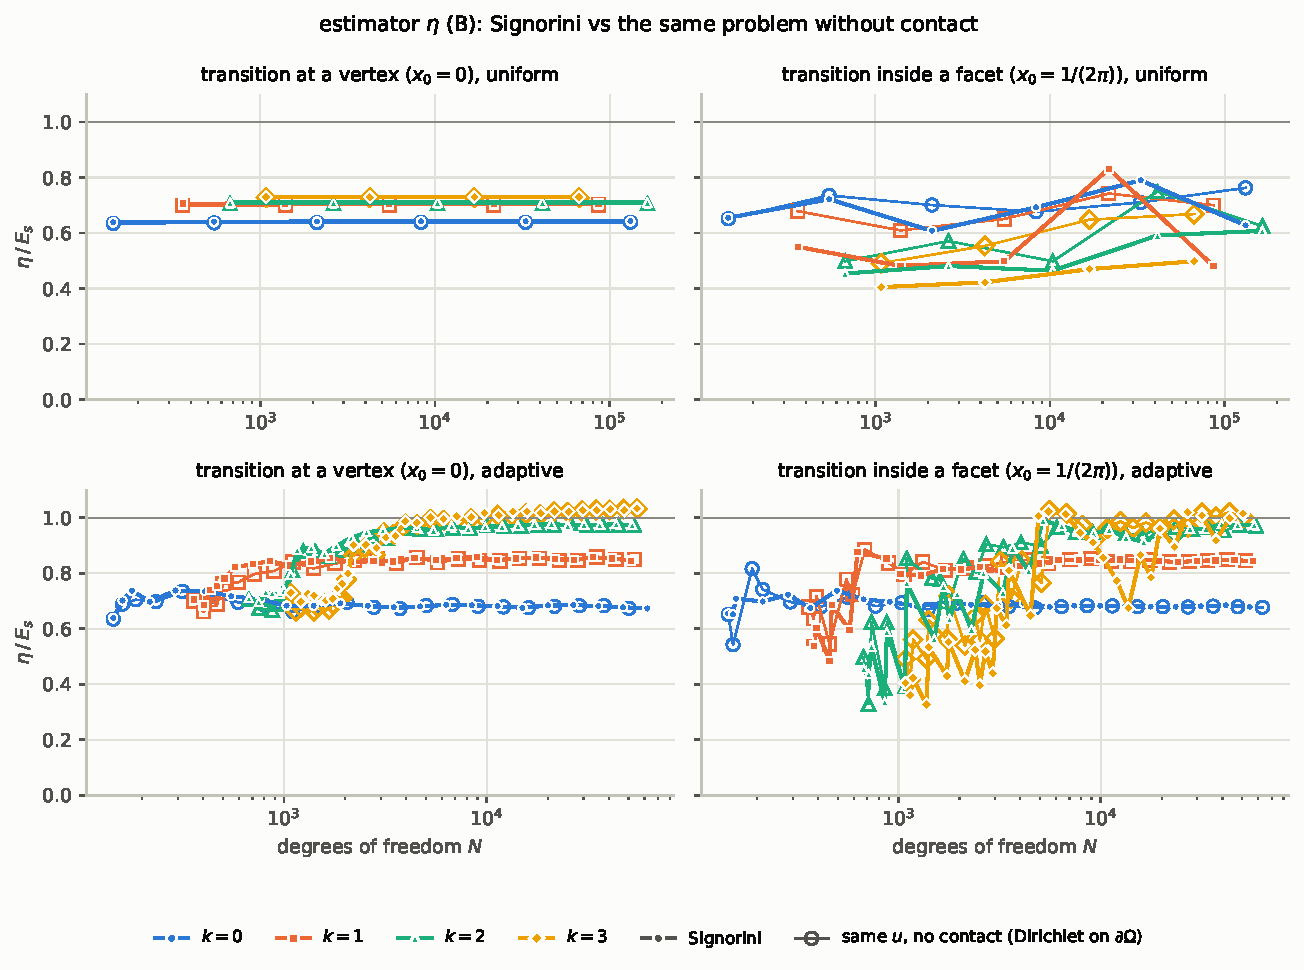
\includegraphics[width=0.92\linewidth]{06_estimators/linear_vs_signorini.pdf}
  \caption{$\eta/E_s$ for Signorini (filled) and for the same $u$ without contact (hollow): $x_0$ a
  node (left) and inside an edge (right), uniform (top) and adaptive (bottom) refinement.}
  \label{fig:linear}
\end{figure}

\subsection{Data not in \texorpdfstring{$\Pk{k}$}{P\_k}}\label{sec:data}

Table~\ref{tab:e8}, Figures~\ref{fig:osc} and~\ref{fig:delta}. In E8 the effectivity is low on the
adaptive meshes and for $k=0$, but not under uniform refinement for $k\ge2$ ($0.71$--$0.73$). On the
adaptive meshes $\delta\approx0.93$--$0.99$, so the constant $1/(1-\delta)$
of~\cite[Thm.~3.9]{mrv} is large. For $k=0$ the oscillation has the size of the error
($\mathrm{osc}/E_s\approx1.1$); for $k\ge1$ on the adaptive meshes it is 2--4 times the error, so it
does not by itself account for what is missing. E6 shows the same pattern for $k=0$
($0.24$--$0.33$ adaptive against $0.63$ uniform, $\delta\approx0.97$--$0.99$) and a much weaker one
for $k=1,2$ ($0.60$--$0.74$ against $0.70$--$0.79$).

\begin{table}[htbp]
\centering\small
\begin{tabular}{@{}lcccccc@{}}
\toprule
 & \multicolumn{3}{c}{adaptive} & \multicolumn{3}{c}{uniform} \\
\cmidrule(lr){2-4}\cmidrule(lr){5-7}
$k$ & $\eta/E_s$ & $\mathrm{osc}/E_s$ & $\delta$ & $\eta/E_s$ & $\mathrm{osc}/E_s$ & $\delta$ \\
\midrule
0 & 0.20--0.21 & 1.13--1.15 & 0.99 & 0.35--0.39 & 0.99--1.05 & 0.97 \\
1 & 0.24--0.29 & 2.05--2.13 & 0.97--0.98 & 0.63--0.69 & 0.45--1.11 & 0.84--0.87 \\
2 & 0.26--0.31 & 2.90--3.05 & 0.95--0.97 & 0.71 & 0.05--0.24 & 0.84 \\
3 & 0.23--0.32 & 3.71--3.99 & 0.93--0.96 & 0.73 & 0.06--0.42 & 0.85 \\
\bottomrule
\end{tabular}
\caption{E8 (BGK 7.2): effectivity, relative oscillation
$\mathrm{osc}:=(\sum_K(h_K/\pi)^2\|f-Q_hf\|_K^2)^{1/2}$ and saturation constant $\delta$. The
values of $\delta$ come from the runs driven by $\tilde\eta$.}
\label{tab:e8}
\end{table}

\begin{figure}[htbp]
  \centering
  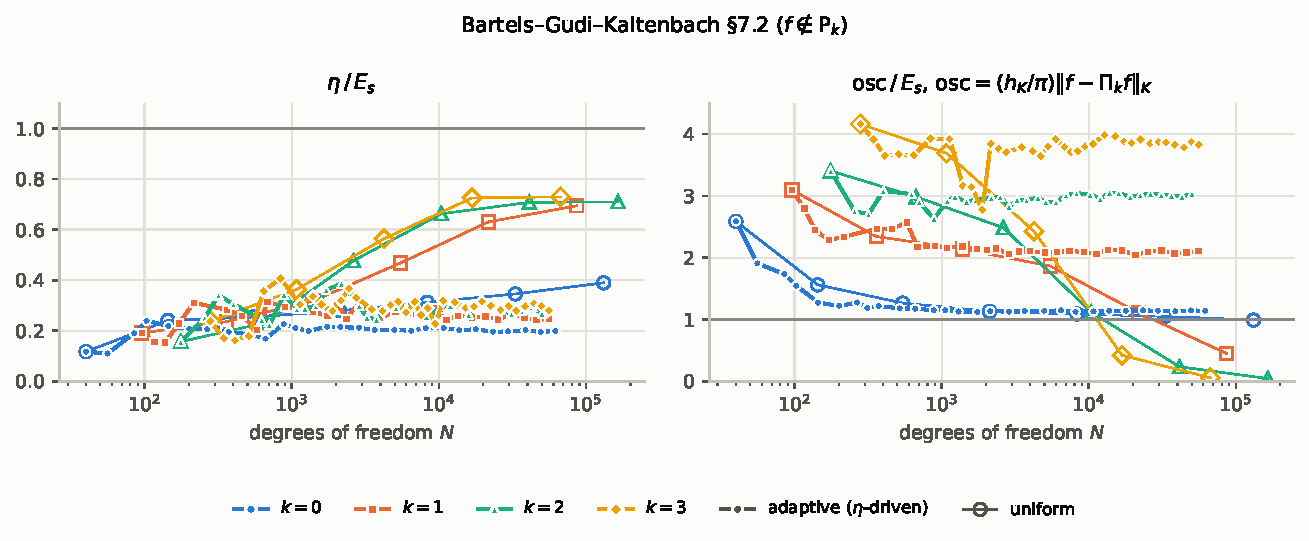
\includegraphics[width=0.92\linewidth]{06_estimators/bgk72_oscillation.pdf}
  \caption{E8: $\eta/E_s$ (left) and $\mathrm{osc}/E_s$ (right); $\eta$-driven adaptive (filled)
  and uniform (hollow) refinement.}
  \label{fig:osc}
\end{figure}

\begin{figure}[htbp]
  \centering
  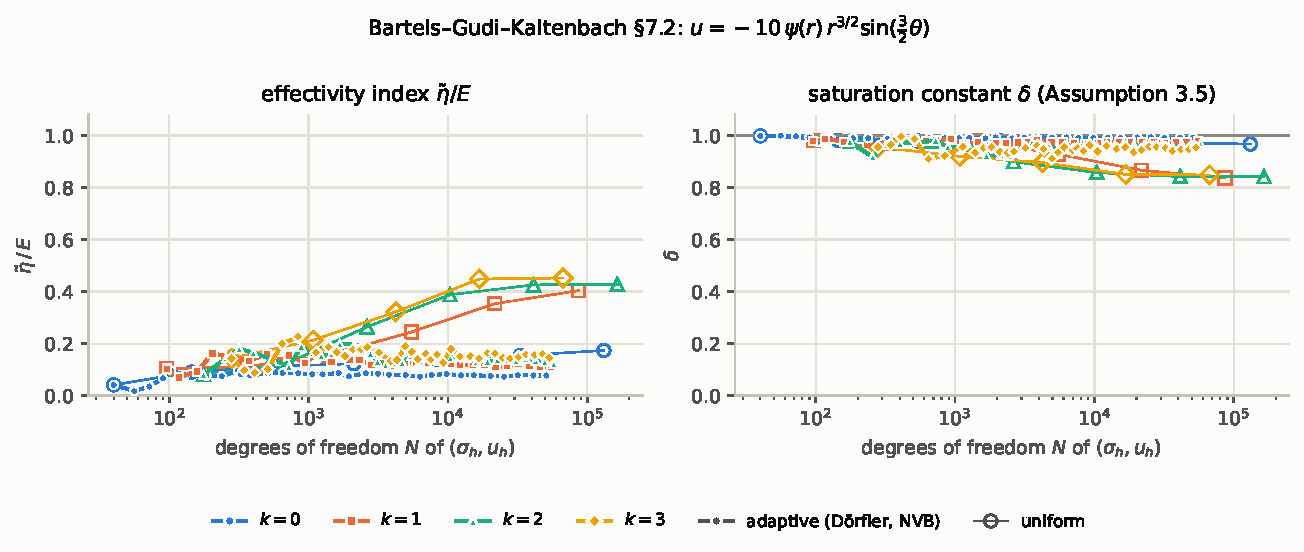
\includegraphics[width=0.92\linewidth]{05_references/bgk72_effectivity.pdf}
  \caption{E8, runs driven by $\tilde\eta$: $\tilde\eta/E$ (left) and the saturation constant
  $\delta$ (right).}
  \label{fig:delta}
\end{figure}

\subsection{Examples without exact solution}\label{sec:unknown}

Table~\ref{tab:unknown}, Figure~\ref{fig:meshes}. In E7 the uniform slope $-0.34$ matches the
reduced rate reported in~\cite{fhs} for their lowest-order DPG method
($(\#\mathcal{T})^{-\alpha/2}$, $\alpha\approx0.7$). Adaptive refinement gives the optimal $-0.98$
for $k=0$ but stays below the optimal rate for $k\ge1$; the meshes refine at the re-entrant corner
and along the circle $|x|=0.8$ where $f$ jumps. In E9 adaptive refinement gives the optimal rate for
every $k$, refining at the junction $(1,0)$ of $\Gamma_D$ and $\Gamma_N$ and at isolated points of
the contact boundary.

\begin{table}[htbp]
\centering\small
\begin{tabular}{@{}lcccc@{}}
\toprule
 & \multicolumn{2}{c}{E7, FHS 4.3} & \multicolumn{2}{c}{E9, BGK 7.3.1} \\
\cmidrule(lr){2-3}\cmidrule(lr){4-5}
$k$ & uniform & adaptive & uniform & adaptive \\
\midrule
0 & $-0.34$ & $-0.98$ & $-0.25$ & $-0.99$ \\
1 & $-0.34$ & $-1.31$ & $-0.25$ & $-1.49$ \\
2 & $-0.34$ & $-1.46$ & $-0.25$ & $-2.03$ \\
3 & $-0.34$ & $-1.47$ & $-0.26$ & $-2.69$ \\
\bottomrule
\end{tabular}
\caption{E7 and E9: slope $s$ of $\eta\sim N^s$. Optimal: $-(k+2)/2$.}
\label{tab:unknown}
\end{table}

\begin{figure}[htbp]
  \centering
  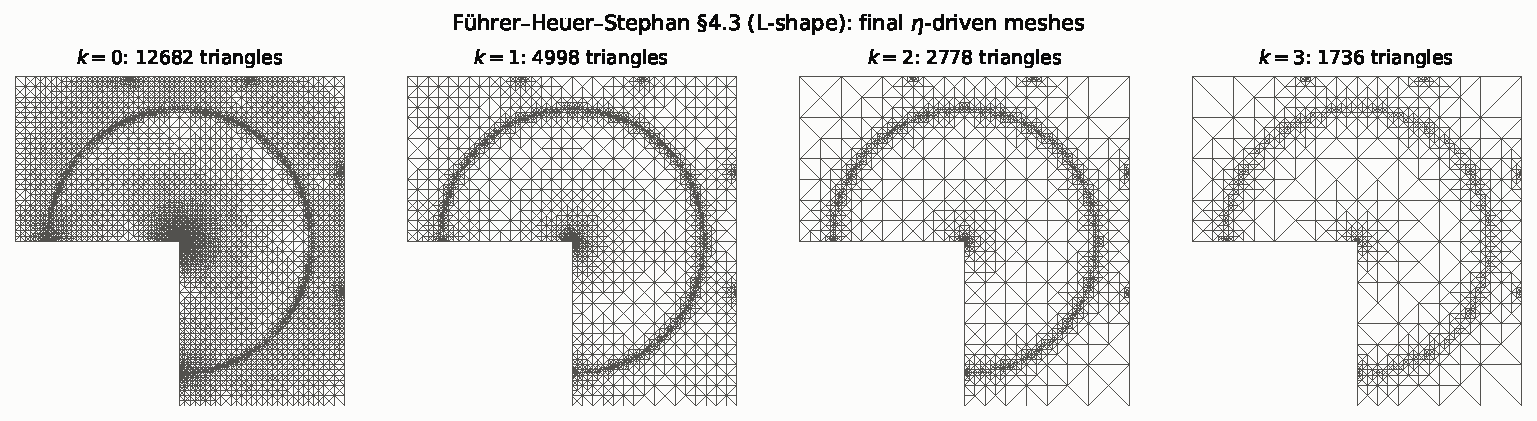
\includegraphics[width=0.9\linewidth]{06_estimators/fhs43_meshes.pdf}\\[2mm]
  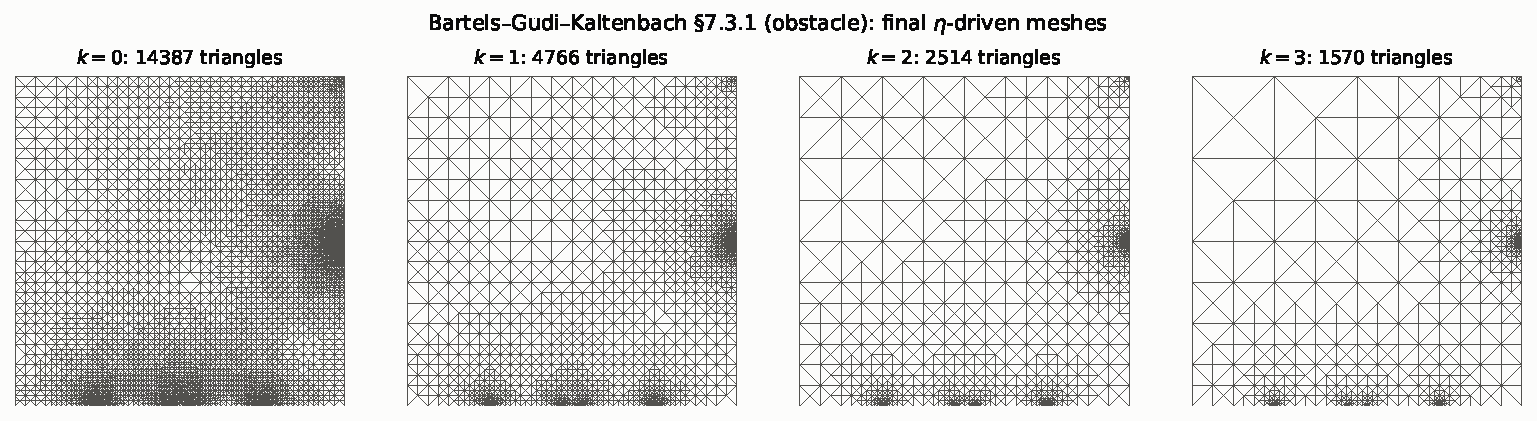
\includegraphics[width=0.9\linewidth]{06_estimators/bgk731_meshes.pdf}
  \caption{Final $\eta$-driven adaptive meshes for E7 (top) and E9 (bottom), $k=0,\dots,3$.}
  \label{fig:meshes}
\end{figure}

\paragraph{Solver.} The active set terminated in every run (at most $44$ iterations from the fully
separated state); no cycling was observed.

\section{Superconvergence at the lowest order}\label{sec:low}

MRV gain \emph{one} order for $p=k+1=1$ instead of two, unless $f\in\Pk0$~\cite[(2.9), (2.15)]{mrv}.
The reason is the bound~\cite[(2.11)]{mrv},
\[
  \|u-\nu_h\|_K \le \tfrac{h_K}{\pi}\bigl(\|q-q_h\|_K+\|\nabla(u-Q^{p+1}_Ku)\|_K\bigr)
  +\|u_h-Q^{p-1}_Ku\|_K+\|u-Q^{p+1}_Ku\|_K ,
\]
in which every term is $O(h^{p+2})$ except the supercloseness $\|u_h-Q^{p-1}_hu\|$, obtained by
duality~\cite{stenberg} on convex domains:
\[
  \|Q^{p-1}_hu-u_h\|\ \lesssim\ h\,\|q-q_h\|+h^{\min(p,2)}\,\|\dive(q-q_h)\|,
  \qquad \dive(q-q_h)=f-Q^{p-1}_hf .
\]
For $p\ge2$ the second term is $h^2O(h^p)$: two orders are gained. For $p=1$ and $f\notin\Pk0$ it is
$hO(h)=O(h^2)$: one order. For $p=1$ and $f\in\Pk0$ it vanishes and $h\|q-q_h\|=O(h^3)$ remains: two
orders. E1 has $f=-2$, so $k=0$ is the third case. Replacing $y^2$ by $y^2\cos(\pi x)$ (same
conditions on $\Gamma_C$, $f=(\pi^2y^2-2)\cos(\pi x)\notin\Pk0$):

\begin{center}\small
\begin{tabular}{@{}llcc@{}}
\toprule
$f$ & $k$ & rates $\|u-u_h\|$ & rates $\|u-\nu_h\|$ \\
\midrule
$-2\in\Pk0$                          & 0 & 0.99,\ 1.00,\ 1.00 & 2.95,\ 2.97,\ 2.99 \\
$(\pi^2y^2-2)\cos(\pi x)\notin\Pk0$  & 0 & 0.98,\ 1.00,\ 1.00 & 2.39,\ 2.21,\ 2.11 \\
$(\pi^2y^2-2)\cos(\pi x)\notin\Pk0$  & 1 & 1.94,\ 1.98,\ 2.00 & 4.01,\ 4.00,\ 4.00 \\
\bottomrule
\end{tabular}
\end{center}
The theory is for the linear problem; with contact this is a numerical observation in a favourable
case (smooth solution, transition at a node).

\section{Open items}\label{sec:open}

\begin{enumerate}
  \item Reliability of $\eta$ for the variational inequality. Even in the linear case MRV's proof
        uses saturation, and E8 shows $\delta$ close to $1$ on adaptive meshes.
  \item \emph{Transition inside an edge.} Under uniform refinement and $k\ge1$, Signorini loses
        up to 30\,\% of effectivity with respect to the same solution without contact (Section~\ref{sec:control}).
        None of the tested contact terms captures it, and where this error is located has not been
        determined.
  \item \emph{Data not in $\Pk{k}$.} The low effectivity on adaptive meshes (E8, E6) is compatible
        with a large saturation constant; the oscillation of $f$ explains it for $k=0$ but
        overshoots for $k\ge1$. The cause is not established.
  \item For $k\ge1$ the Bernstein cone is only sufficient for $\sigma_h\cdot n\ge0$; its effect on
        accuracy near transitions has not been quantified.
  \item E7 with $k\ge1$: adaptive rates below optimal, presumably limited by the jump of $f$ along
        $|x|=0.8$.
  \item Variable diffusion coefficient, robustness in the reaction coefficient (FHS 4.4), 3D.
\end{enumerate}

\paragraph{Code.} The Julia package \texttt{SignoriniPostprocessing.jl} (Gridap) accompanies this
note; its studies (convergence, adaptivity, references, estimators, control without contact)
reproduce all tables and figures.

\begin{thebibliography}{9}
\bibitem{bgk} S.~Bartels, T.~Gudi, A.~Kaltenbach. A priori and a posteriori error identities for
  the scalar Signorini problem. arXiv:2407.10912 (2024).
\bibitem{fhs} T.~Führer, N.~Heuer, E.~P.~Stephan. On the DPG method for Signorini problems.
  arXiv:1609.00765 (2016).
\bibitem{hik} M.~Hintermüller, K.~Ito, K.~Kunisch. The primal-dual active set strategy as a
  semismooth Newton method. \emph{SIAM J.\ Optim.} 13 (2003) 865--888.
\bibitem{mrv} I.~Muga, S.~Rojas, P.~Vega. An adaptive superconvergent mixed finite element method
  based on local residual minimization. \emph{SIAM J.\ Numer.\ Anal.} 61(5) (2023) 2084--2105,
  doi:10.1137/22M1526307. Equation numbers refer to this version.
\bibitem{stenberg} R.~Stenberg. Postprocessing schemes for some mixed finite elements.
  \emph{ESAIM: M2AN} 25 (1991) 151--167.
\bibitem{wang} Q.~Wang, J.~Hu, G.~Zhou. The mixed method with two Lagrange multiplier formulations
  for the Signorini problem. \emph{J.\ Comput.\ Appl.\ Math.} 452 (2024) 116115.
\end{thebibliography}

\end{document}
